\documentclass[UTF8]{ctexart}
\usepackage{xcolor}
\usepackage{graphicx}
\usepackage{listings}
\usepackage[hidelinks]{hyperref}
\usepackage[left=1.25in,right=1.25in,top=1in,bottom=1in]{geometry}
\usepackage{ctex}
\usepackage{multirow}
\usepackage{booktabs}
\usepackage{pythonhighlight}
\usepackage{float}
\usepackage{amsmath}


\title{人工智能及其应用实验报告}
\author{花国栋}

\begin{document}
    \zihao{5}
    \maketitle
    \tableofcontents
    \newpage
    \section{实验简介}
        \subsection{实验目的}
        \begin{enumerate}
            \item 掌握python的基础数学操作与科学计算库。
            \item 学习数据预处理的各种基本方法。
            \item 了解SVM与PCA原理,掌握实际的代码应用以及如何优化超参数。
        \end{enumerate}
        \subsection{实验要求}
        选取合适的算法对给定的数据集训练与测试,进行参数优化,计算算法评价的指标。
        \subsection{研究方法}
        首先读取数据,然后统计缺失值,本实验中无缺失值,故接下来拆分特征列与目标列,然后进行数据集划分,其中
        训练集占比80\%,测试集占比20\%,接着对特征进行PCA降维,然后进行数据的归一化,最后构建SVM分类模型,
        通过网格搜索与10折交叉验证寻找最佳分类器,接着再用最佳分类器在测试集上测试,使用混淆矩阵与分类报告进行
        算法模型的分类效果的评估。
        \subsection{数据集介绍}
        该数据集一共有11个特征值和一个目标值,共1599组,分别为:

        1-固定酸度 2-挥发性酸度 3-柠檬酸 4-残留糖 5-氯化物 6-游离二氧化硫
        7-总二氧化硫 8-密度 9-pH 10-硫酸盐 11-醇 12-质量
        \begin{figure}[htbp]
            \centering
            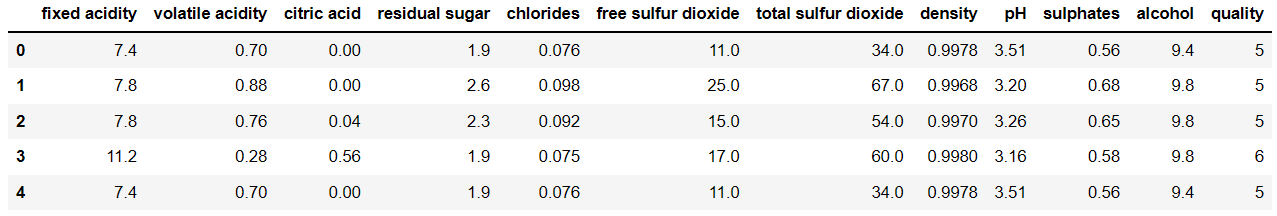
\includegraphics[scale=0.5]{data_head.png}
            \caption{数据前五行}
            \label{figure1}
        \end{figure}
        \subsection{技术工具}
        \begin{itemize}
            \item Python版本 3.9.15
            \item 代码编辑器 Visual Studio Code
            \item 虚拟环境配置工具 Anaconda
            \item 辅助工具 Jupyter Notebook
        \end{itemize}
    \section{实验步骤及算法简述}
        \subsection{导入实验相关库}
            \begin{python}
import pandas as pd
import numpy as np
from sklearn.preprocessing import MinMaxScaler
from sklearn import svm
from sklearn.model_selection import train_test_split
from sklearn.model_selection import GridSearchCV
from sklearn.decomposition import PCA
from sklearn.metrics import confusion_matrix,classification_report 
from sklearn.metrics import precision_recall_curve
import matplotlib.pyplot as plt               
            \end{python}
        \subsection{读取数据}
        使用pandas库的read\_csv()方法读取数据,并进行是否有缺失值的判断。
            \begin{python}
data=pd.read_csv('winequality-red.csv',sep=';') #从文件中读取data
#print(data.isnull().sum())  #统计有几个缺失值,为0所以不做后续处理
            \end{python}
        \subsection{拆分特征列与目标列}
        从之前数据集的组成可以看到,label=quality的那一列为目标列,剩余的则为特征列,由于quality分布区间为0-10,
        分布太广,且过于细致,所以将质量分为两个等级:劣质,优质。将多分类问题转化为二分类问题,也有利于
        缓解因为数据集过少训练出的模型不准确的问题。
            \begin{python}
X = data.drop(labels='quality',axis=1).copy()	#X是特征列
y = data['quality'].copy()	                    #y是目标列
for i in range(1599):
    y[i]=np.where(y[i]<=5,-1,1)#将Quality大于5为优质,定为1,反之则为劣质,定为-1
            \end{python}
        \subsection{划分训练集与测试集}
        用sklearn库的train\_test\_split的方法按照8:2的比例划分训练集与测试集,随机种子random\_state设为固定值0,
        这是为了让后面的PCA降维时对同一划分的数据集进行手动调参。
            \begin{python}
X_train,X_test,y_train,y_test = train_test_split(X,y,test_size=0.2,random_state=0) 
            \end{python}
        \subsection{PCA降维}
        主成分分析(Principal Component Analysis,PCA)算法能够将高维问题简化成低维问题,具有简单、快速,且主成分之
        间相互正交,可消除原始数据成分间的影响。观察原数据集结合常识直觉,可以发现pH与固定酸度、挥发性酸度等都有相关性,
        故可以借助PCA降维,去除噪声和不重要的特征。在random\_state不变的情况下,对维度n\_components进行手动选择,
        可以发现维度在7时效果最好,这也符合数学直觉,当维度过低时,特征损失较大,当维度过高时,PCA效果不明显。
            \begin{python}
pca=PCA(n_components=7)
pca.fit(X_train)
X_train_pca=pca.transform(X_train)
X_test_pca=pca.transform(X_test)            
            \end{python}
        \subsection{归一化}
        使用了sklearn库的MinMaxScaler方法对原始数据进行线性变换,变换到[0,1]区间。计算公式为:
        \begin{equation}
            X_{scaled}=\frac{X-\min }{\max -\min }\left(n e w_{-} \max -n e w_{-} \min \right)+n e w_{-} \min
        \end{equation}
            \begin{python}
X_scaler = MinMaxScaler()
X_train_scaled=X_scaler.fit_transform(X_train_pca)
X_test_scaled=X_scaler.transform(X_test_pca)
            \end{python}
        \subsection{网格搜索\&交叉验证来最优化SVM模型}
        分类问题选用SVM模型,sklearn库中的SVC方法。支持向量机(Support Vector Machine,SVM),
        通俗来讲,它是一种二类分类模型,其基本模型定义为特征空间上的间隔最大的线性分类器,其学习策略便是间隔最大化,
        最终可转化为一个凸二次规划问题的求解。

        在使用SVM对数据进行训练的时候,为了使得在模型准确度达到一定的要求的条件下,模型的泛化能力尽量更好,
        防止在训练过程中模型的过拟合。因此我们需要不断的调整SVC()方法中gamma和C的值,
        并对数据不断地进行交叉验证,以找到合适的gamma和C的值。

        参数C的作用:C是惩罚系数,理解为调节优化方向中两个指标(间隔大小,分类准确度)偏好的权重,
        即对误差的宽容度。C越高,说明越不能容忍出现误差,容易过拟合;
        C越小,容易欠拟合。C过大或者是过小,泛化能力都会变差。

        参数gamma的作用:gamma是选择RBF函数作为kernel后,该函数自带的一个参数。
        隐含地决定了数据映射到新的特征空间后的分布,gamma越大,支持向量越少;gamma越小,支持向量越多。
        支持向量的个数影响训练与预测的速度。

        网格搜索(Grid Search)就是在C,gamma组成的二维参数矩阵中,依次实验每一对参数的效果,可以得到全局最优。

        k折交叉验证(K-fold Cross-Validation),将训练集分为k份,其中k-1份为训练集,剩下一份为验证集,用
        训练集训练模型,再在验证集上进行测试,获得其在验证集上的Accuracy,k次之后取平均。

        使用sklearn库的GridSearchCV方法,进行网格搜索结合k折交叉验证获得最好的超参数gamma和C后,
        代入模型,将训练集上训练模型。
            \begin{python}
params = {
    'gamma':[0.01, 0.1, 0.5, 1, 2, 10, 100],
    'C': [0.01, 0.1, 0.5, 1, 2, 10, 100]
    }
clf=svm.SVC()#选用SVM模型
grid=GridSearchCV(clf,params,cv=10,n_jobs=-1)
grid.fit(X_train_scaled,y_train)
            \end{python}
        % \newpage
        \subsection{结果展示}
            \begin{python}
y_pred=grid.predict(X_test_scaled)
print('最佳分类器:',grid.best_estimator_)
print("混淆矩阵\n",confusion_matrix(y_test,y_pred))
print("分类报告\n",classification_report(y_test,y_pred))
            \end{python}
            \begin{figure}[htbp]
                \centering
                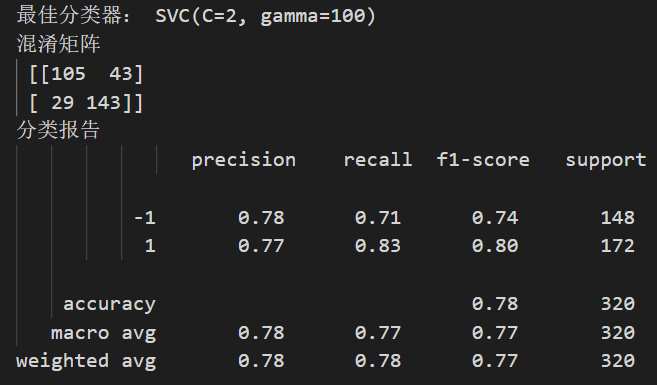
\includegraphics[scale=1]{result.png}
                \caption{分类器在测试集上的混淆矩阵与分类报告}
                \label{figure2}
            \end{figure}
            \subsection{PR曲线绘制}
            PR曲线中的P代表的是Precision(查准率),R代表的是Recall(查全率),
            其代表的是精准率与召回率的关系,一般情况下,将Recall设置为横坐标,Precision设置为纵坐标。
            使用的是matplotlib库中的绘图方法。
            \begin{python}
precision, recall, thresholds = precision_recall_curve(y_test, y_pred)
plt.figure()
plt.plot(recall, precision)
plt.title('Precision Recall Curve')
plt.xlabel('Recall')
plt.ylabel('Precision')
plt.show()
            \end{python}
            \begin{figure}
                \centering
                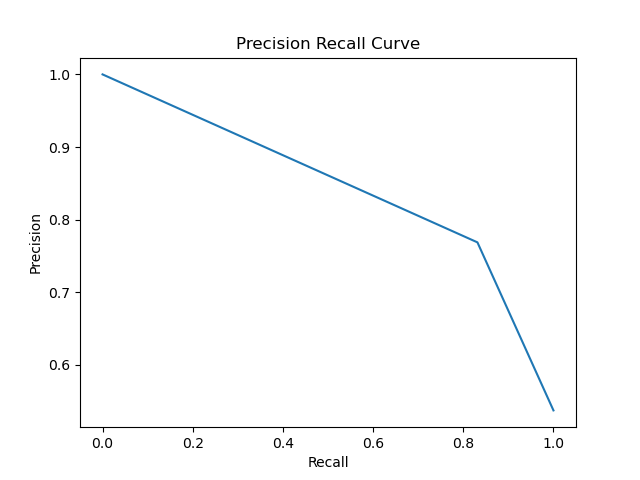
\includegraphics[scale=0.8]{PR.png}
                \caption{PR曲线}
                \label{figure2}
            \end{figure}
    \newpage
    \section{结果说明}
    \begin{table}[htbp]
        \centering
        \caption{混淆矩阵}
        \begin{tabular}{|c|c|c|c|} 
        \toprule
        \multicolumn{2}{|c|}{\multirow{2}{*}{混淆矩阵}} & \multicolumn{2}{c|}{预测结果}  \\ 
        \cline{3-4}
        \multicolumn{2}{|c|}{}                      & 正例      & 反例               \\ 
        \hline
        \multirow{2}{*}{真实情况} & 正例                  & TP(真正例) & FN(假反例)          \\ 
        \cline{2-4}
                                & 反例                  & FP(假正例) & TN(真反例)          \\
        \bottomrule
        \end{tabular}
    \end{table}
    
    \noindent
    查准率:
    \begin{equation}
        \text { Precision }=\frac{\text { TP } }{\text { TP}+\text { FP }}
    \end{equation}
    查全率:
    \begin{equation}
        \text { Recall }=\frac{\text { TP}}{\text { TP }+\text { FN }}
    \end{equation}
    准确度:
    \begin{equation}
        \text { Accuracy }=\frac{T P+T N}{T P+F P++T N+F N}
    \end{equation}
    F1 score:
    \begin{equation}
        \mathrm{F} 1=2 \times \frac{\text { Precision } * \text { Recall }}{\text { Precision }+\text { Recall }}
    \end{equation}
    \section{实验源码}
    \begin{python}
import pandas as pd
import numpy as np
from sklearn.preprocessing import MinMaxScaler
from sklearn import svm
from sklearn.model_selection import train_test_split
from sklearn.model_selection import GridSearchCV
from sklearn.decomposition import PCA
from sklearn.metrics import confusion_matrix,classification_report
from sklearn.metrics import precision_recall_curve
import matplotlib.pyplot as plt

#读取数据
data=pd.read_csv('winequality-red.csv',sep=';') #从文件中读取data
#print(data.isnull().sum())  #统计有几个缺失值,为0所以不做后续处理

#拆分特征列与目标列
X = data.drop(labels='quality',axis=1).copy()	#X是特征列
y = data['quality'].copy()	                    #y是目标列
for i in range(1599):
    y[i]=np.where(y[i]<=5,-1,1)#将Quality大于5为优质,定为1,反之则为劣质,定为-1

#8:2划分训练集与测试集
X_train,X_test,y_train,y_test = train_test_split(X,y,test_size=0.2,random_state=0)      

#PCA降维
pca=PCA(n_components=7)
pca.fit(X_train)
X_train_pca=pca.transform(X_train)
X_test_pca=pca.transform(X_test)

#归一化
X_scaler = MinMaxScaler()
X_train_scaled=X_scaler.fit_transform(X_train_pca)
X_test_scaled=X_scaler.transform(X_test_pca)

#网格搜索交叉验证来调整SVC函数中的超参数
params = {
    'gamma':[0.01, 0.1, 0.5, 1, 2, 10, 100],
    'C': [0.01, 0.1, 0.5, 1, 2, 10, 100]
    }
clf=svm.SVC()#选用SVM模型
grid=GridSearchCV(clf,params,cv=10,n_jobs=-1)
grid.fit(X_train_scaled,y_train)

#结果展示
y_pred=grid.predict(X_test_scaled)
print('最佳分类器:',grid.best_estimator_)
print("混淆矩阵\n",confusion_matrix(y_test,y_pred))
print("分类报告\n",classification_report(y_test,y_pred))

#PR曲线
precision, recall, thresholds = precision_recall_curve(y_test, y_pred)
plt.figure()
plt.plot(recall, precision)
plt.title('Precision Recall Curve')
plt.xlabel('Recall')
plt.ylabel('Precision')
plt.show()        
    \end{python}
\end{document}